% Copyright (c) 20090-2014 by the University of Waikato, Hamilton, NZ. 
% This work is made available under the terms of the 
% Creative Commons Attribution-ShareAlike 3.0 license, 
% http://creativecommons.org/licenses/by-sa/3.0/. 
%
% Version: $Revision$

\chapter{Classification and Regression}
\label{classification_and_regression}
WEKA's main strength lies in its large number of classification and regression
schemes. Most of the documentation will cover this functionality therefore.

We start out with some basic WEKA functionality, like loading and
preprocessing data, building models and evaluating them. That includes
visualization of the results and models as well. After that we will cover more
advanced features like learning
curves, experiment generation and evaluation, optimization of classifiers and
also the current provenance support in ADAMS.

\newpage
\section{Basic}
In this section we describe how to perform basic WEKA functionality that you are
used to perform with the Explorer, but in the workflow context. Instead of
having to repeat the same steps, like loading and preprocessing data, whenever
you update your data, a flow allows you to define the steps apriori and then merely
re-execute them time and time again. Also, flows make it very easy to
\textit{document} all the steps that you perform, not just merely recording what
you are doing.

\subsection{Loading data}
Before we can build any models, we have to have data at hand, of course. So the
first step will be to obtain data from somewhere, whether that is by loading a
local dataset or by downloading a remote dataset.

To start, we will be loading files that are stored locally. The actor used for
loading datasets is the \textit{WekaFileReader} transformer. This actor does not
have an option for the file to load. Instead, it expects a file name, string or
URL object to arrive at its input port. In order to supply a local file, we use
the \textit{SingleFileSupplier} source, which allows us to specify a single file
that gets forwarded in the flow. If required, one can also use the
\textit{MultiFileSupplier} or \textit{DirectoryLister}
sources\footnote{adams-weka-crossvalidate\_classifier\_multiple\_datasets.flow},
which can forward multiple file names instead of just one. The latter one is
especially handy, if the files are not known in advance, e.g., generated on the
fly. In order to display the loaded data, we use the
\textit{WekaInstancesDisplay} sink actor, which displays the data in a nice
tabular format. Figure \ref{basic-load_local_dataset} shows the flow for loading
the dataset and Figure \ref{basic-load_local_dataset-output} the generated
output.

\begin{figure}[ht]
  \begin{minipage}[t]{0.5\linewidth}
    \centering
    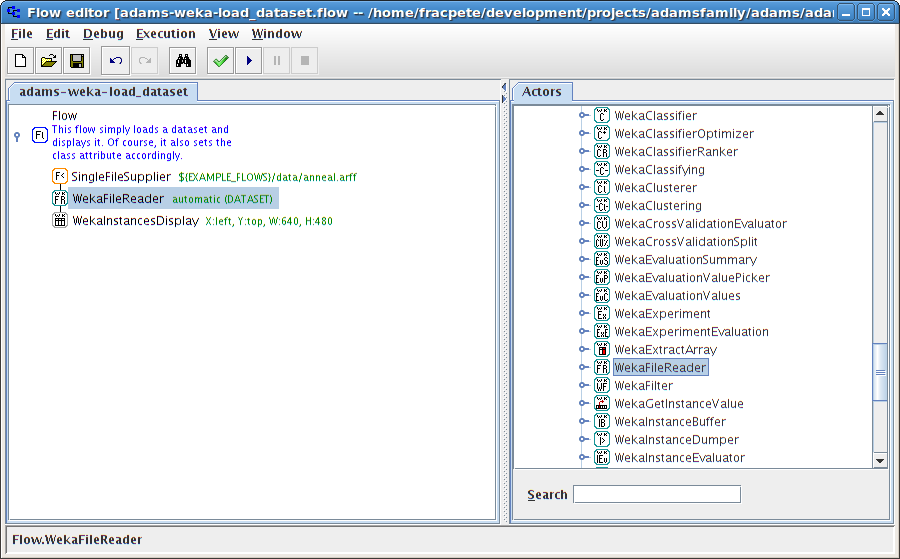
\includegraphics[width=6.0cm]{images/basic-load_local_dataset.png}
    \caption{Flow for loading a local dataset.}
    \label{basic-load_local_dataset}
  \end{minipage}
  \hspace{0.5cm}
  \begin{minipage}[t]{0.5\linewidth}
    \centering
    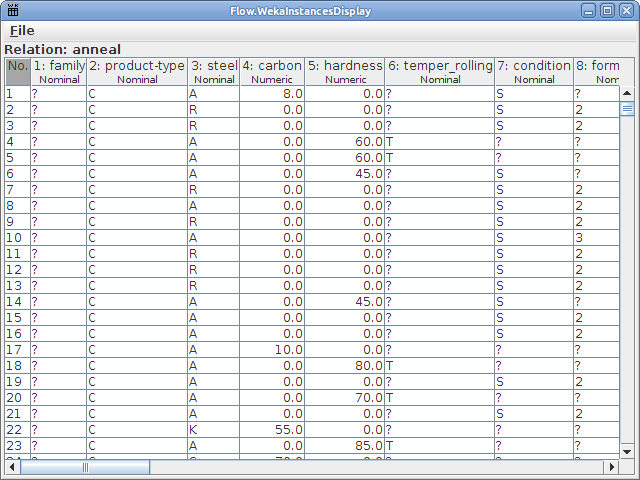
\includegraphics[width=5.0cm]{images/basic-load_local_dataset-output.png}
    \caption{The dataset that got loaded from disk.}
    \label{basic-load_local_dataset-output}
  \end{minipage}
\end{figure}

In this example\footnote{adams-weka-load\_dataset.flow} we let the
\textit{WekaFileReader} determine the correct file loader automatically, based
on the file extension. If this automatic determination should fail, you can
always check the ``useCustomLoader'' checkbox and then configure the appropriate
loader yourself.

Another feature of this actor is the ability to output the dataset row by row
(option ``incremental''). This is very handy in case of very large files, where
loading into memory could pose a problem. Even though the incremental feature
works for any file type that WEKA can read, truly incremental, i.e.,
memory-efficient, loading is only possible if the underlying loader also
supports incremental loading. In any other case, the dataset gets loaded fully
into memory before being forwarded row by row.

Nowadays, a lot of data is available online. Instead of relying on local files,
one can use the flow also to download remote files. Some of the WEKA file
loaders, like the \textit{ArffLoader}, natively support the download via a URL.
Figure \ref{basic-download_dataset} shows a
flow\footnote{adams-all-weka\_dataset\_download.flow} that downloads (and
displays) an ARFF file available from a URL that was supplied by the
\textit{URLSupplier}. If the required dataset is encapsulated in an
archive, e.g., a ZIP file and not just compressed with GZIP, then one has to
download the archive first and extract the correct file before working with it.
The flow\footnote{adams-all-weka\_dataset\_download2.flow} in Figure
\ref{basic-download_dataset2} downloads an archive from WEKA's sourceforge.net
web site\footnote{WEKA on sourceforge.net:
\url{http://sourceforge.net/projects/weka/}{}} using the \textit{DownloadFile}
sink and extracts all the datasets which filename fit a regular expression. The
extracted files are then displayed in a \textit{HistoryDisplay} sink.

\begin{figure}[ht]
  \begin{minipage}[t]{0.5\linewidth}
    \centering
    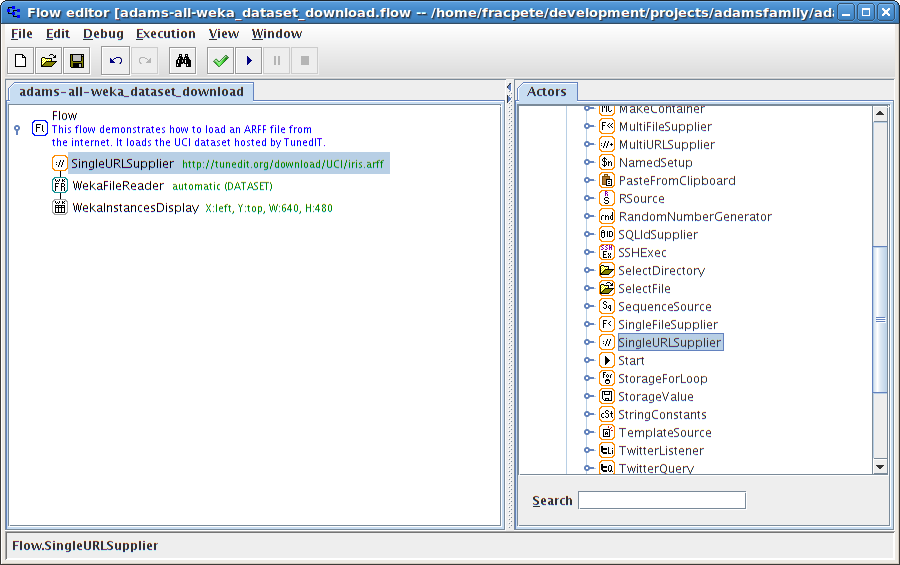
\includegraphics[width=5.5cm]{images/basic-download_dataset.png}
    \caption{Flow for loading a local dataset.}
    \label{basic-download_dataset}
  \end{minipage}
  \hspace{0.5cm}
  \begin{minipage}[t]{0.5\linewidth}
    \centering
    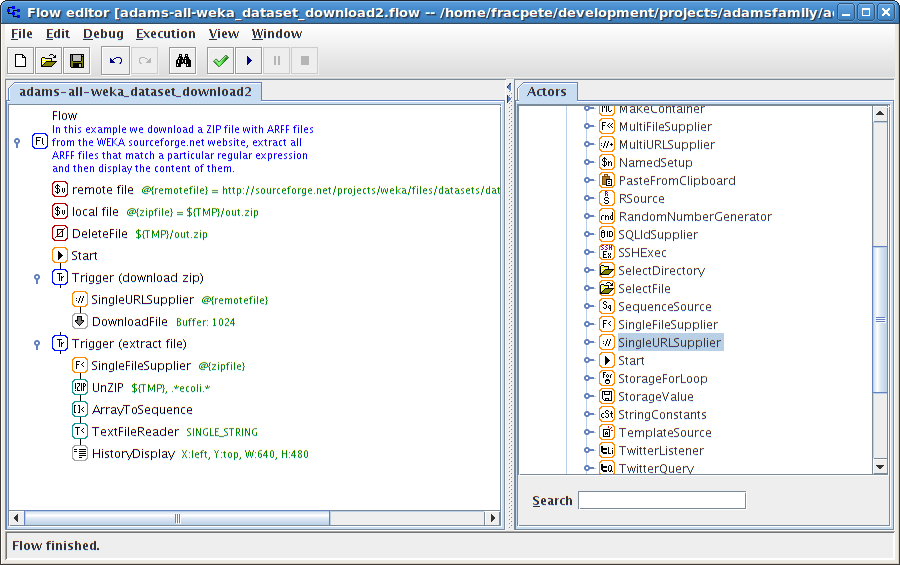
\includegraphics[width=6.0cm]{images/basic-download_dataset2.png}
    \caption{The dataset that got loaded from disk.}
    \label{basic-download_dataset2}
  \end{minipage}
\end{figure}

Finally, artificial data can be generated within ADAMS as well. Using the
\textit{WekaDataGenerator} source, any WEKA data generator can be used to output
data. The flow\footnote{adams-weka-data\_generator.flow} depicted in Figure
\ref{basic-datagenerator} generates a small dataset using the ``Agrawal'' data
generator.

\begin{figure}[htb]
  \centering
  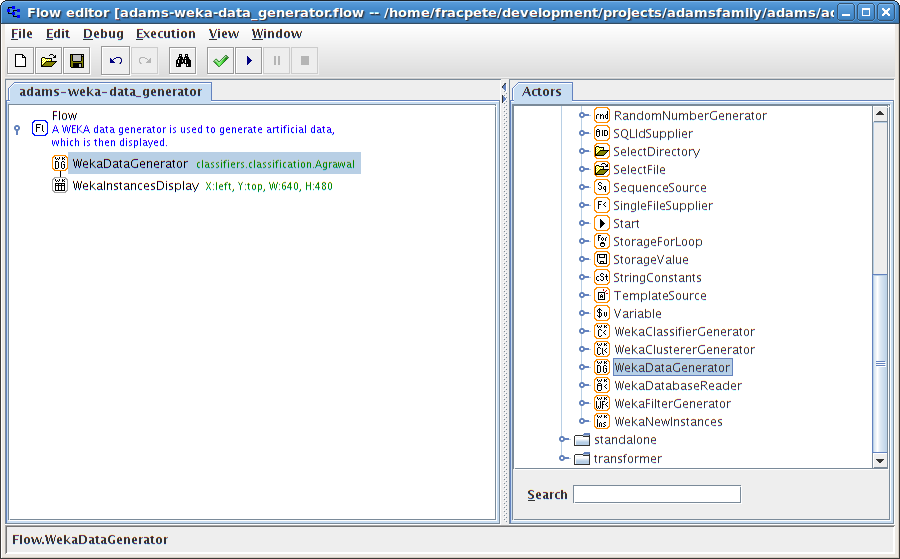
\includegraphics[width=6.0cm]{images/basic-datagenerator.png}
  \caption{Flow for generating and displaying an artificial dataset.}
  \label{basic-datagenerator}
\end{figure}

\subsection{Building models}
After having sorted out the loading of the data, it is time to check out how to
build models. Since we are using supervised algorithms, we have to make sure
that the datasets have a class attribute set. The \textit{WekaClassSelector}
actor allows the setting of the class attribute, in the default setting it
simply uses the last attribute as the class attribute. With the
\textit{WekaTrainClassifier} actor you can choose a callable classifier to be built. 
You define a callable classifier by adding a \textit{WekaClassifierSetup} source
to the \textit{CallableActors} standalone, which you then reference in your 
\textit{WekaTrainClassifier} actor.
By default, the \textit{WekaTrainClassifier} actor outputs a container that comprises
the built model and the header of the training set. In order to extract either
of the container items, you need to use the \textit{ContainerValuePicker}
control actor. Figure \ref{basic-building_model1-flow} demonstrates how to train
a J48 classifier on dataset and then displaying the built model (see Figure
\ref{basic-building_model1-output})\footnote{adams-weka-build\_classifier-output\_only\_model.flow}.

\begin{figure}[ht]
  \begin{minipage}[t]{0.5\linewidth}
    \centering
    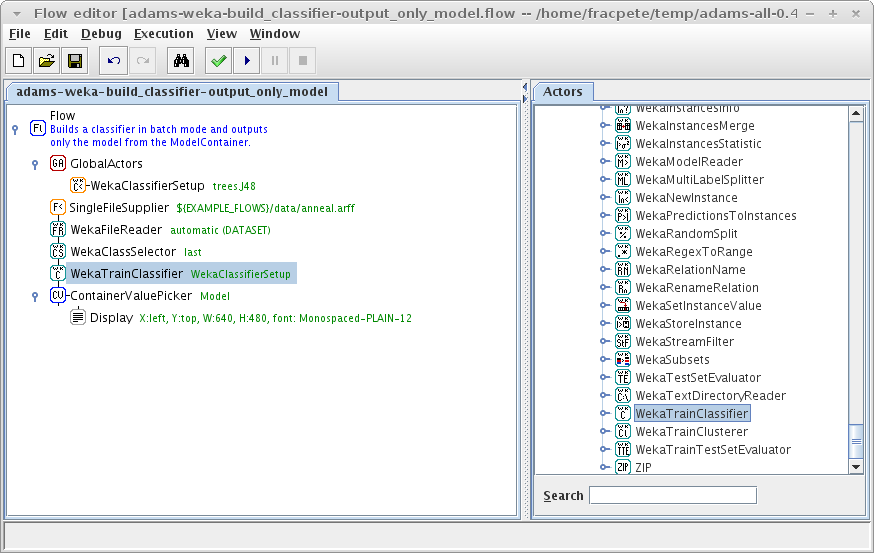
\includegraphics[width=6.0cm]{images/basic-building_model1-flow.png}
    \caption{Flow for building J48 model on a dataset and outputting the model.}
    \label{basic-building_model1-flow}
  \end{minipage}
  \hspace{0.5cm}
  \begin{minipage}[t]{0.5\linewidth}
    \centering
    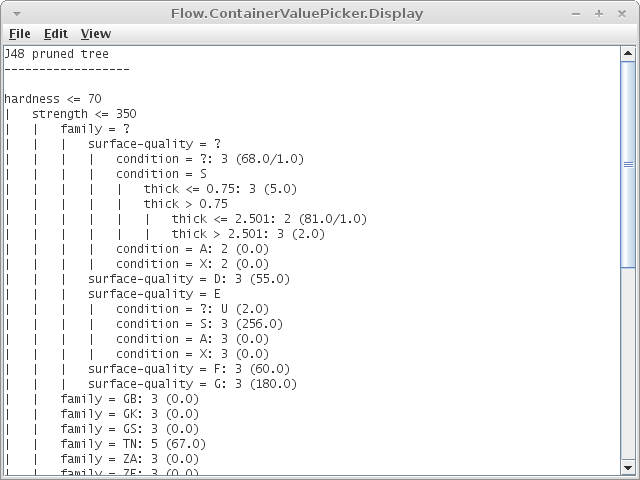
\includegraphics[width=5.5cm]{images/basic-building_model1-output.png}
    \caption{J48 model output.}
    \label{basic-building_model1-output}
  \end{minipage}
\end{figure}

A built model can be saved to disk (and then re-used later) using the
\textit{WekaModelWriter}. The file generated can also be loaded in the WEKA
Explorer again and applied to another test set
there\footnote{adams-weka-build\_classifier-save\_model.flow}.

\subsection{Preprocessing}
A very important, but often underrated step is preprocessing. Unless your data
is properly cleaned up and in the right format, your models will not be very
meaningful. Preprocessing steps can be done within the flow using the
\textit{WekaFilter} transformer, which wraps around a single WEKA filter. One
either chains multiple actors together or uses the
\textit{weka.filters.MultiFilter} meta-filter to executed several filter
sequentially in a single actor.

In Figure \ref{basic-preprocessing_flow} we are investigating the impact of
preprocessing on the ``slug'' dataset \cite{slug}. The
flow\footnote{adams-weka-filter\_data.flow} cross-validates
\textit{LinearRegression} on the original and log-transformed data. The
log-transformed data is generated by applying the \textit{AddExpression} filter
on each of the two attributes of the dataset and then deleting the original
ones. In each case, original or preprocessed, it displays the evaluation summary
and classifier errors.

\begin{figure}[htb]
  \centering
  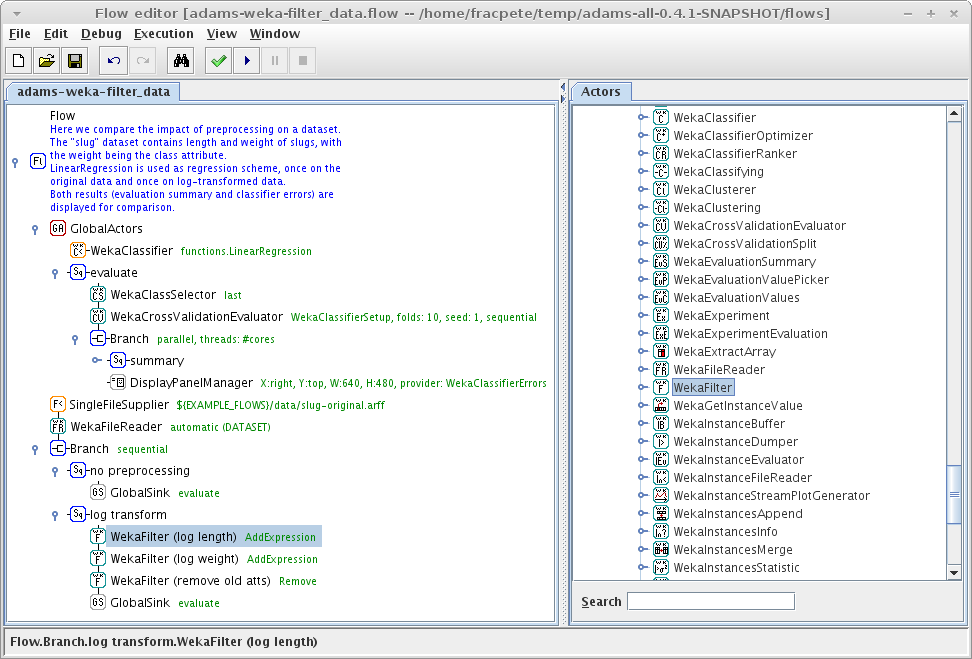
\includegraphics[width=7.0cm]{images/basic-preprocessing_flow.png}
  \caption{Flow for comparing results generated from original and preprocessed
  ``slug'' data \cite{slug}.}
  \label{basic-preprocessing_flow}
\end{figure}

Figures \ref{basic-preprocessing_summary-original} and
\ref{basic-preprocessing_summary-log} show the evaluation summary, for the
original and the log-transformed data. The log-transformed dataset gets not
only a better correlation coefficient, but also smaller errors.

\begin{figure}[ht]
  \begin{minipage}[t]{0.5\linewidth}
    \centering
    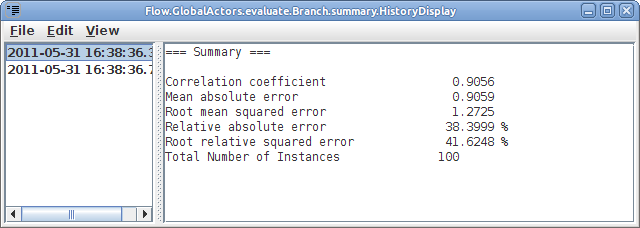
\includegraphics[width=5.5cm]{images/basic-preprocessing_summary-original.png}
    \caption{Evaluation summary on ``slug'' dataset (original).}
    \label{basic-preprocessing_summary-original}
  \end{minipage}
  \hspace{0.5cm}
  \begin{minipage}[t]{0.5\linewidth}
    \centering
    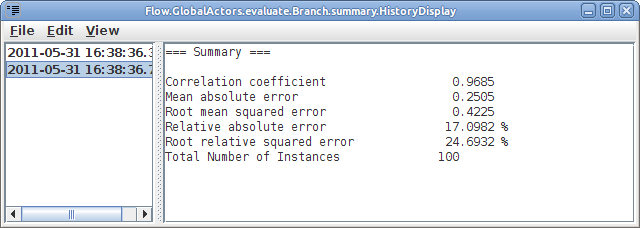
\includegraphics[width=5.5cm]{images/basic-preprocessing_summary-log.png}
    \caption{Evaluation summary on ``slug'' dataset (log-transformed).}
    \label{basic-preprocessing_summary-log}
  \end{minipage}
\end{figure}

Figures \ref{basic-preprocessing_errors-original} and
\ref{basic-preprocessing_errors-log} display the classifier errors. It is
obvious from the funy log-shaped curve, that LinearRegression built on the
original data is not a very good model. Something that is not so obvious by just
looking at the correlation coefficient: 0.9056 is not bad.

\begin{figure}[ht]
  \begin{minipage}[t]{0.5\linewidth}
    \centering
    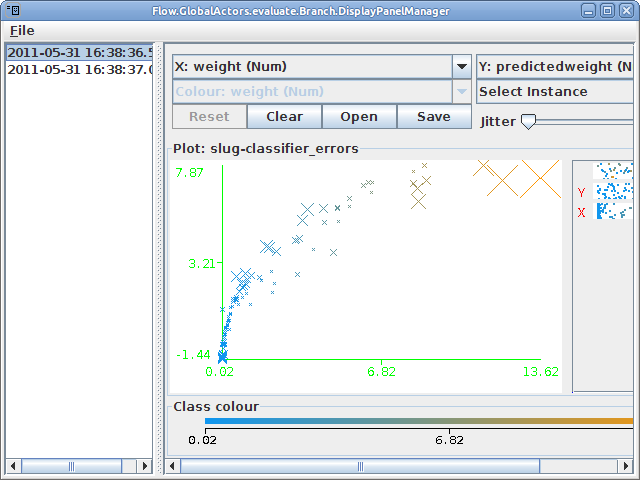
\includegraphics[width=5.5cm]{images/basic-preprocessing_errors-original.png}
    \caption{Classifier errors on ``slug'' dataset (original).}
    \label{basic-preprocessing_errors-original}
  \end{minipage}
  \hspace{0.5cm}
  \begin{minipage}[t]{0.5\linewidth}
    \centering
    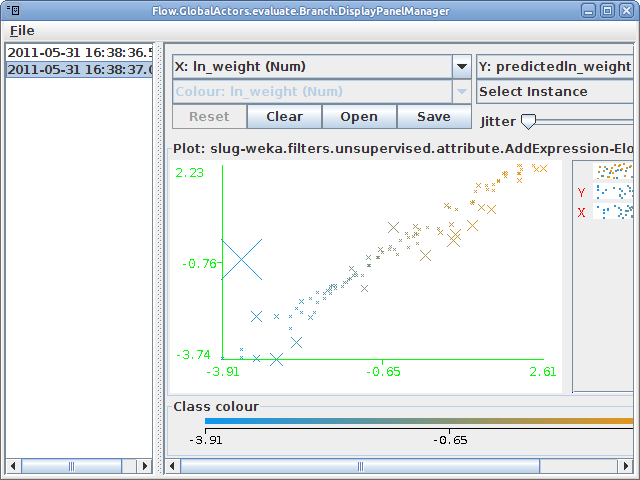
\includegraphics[width=5.5cm]{images/basic-preprocessing_errors-log.png}
    \caption{Classifier errors on ``slug'' dataset (log-transformed).}
    \label{basic-preprocessing_errors-log}
  \end{minipage}
\end{figure}

This flow can be quickly extended to accommodate other preprocessing techniques,
all very easily comparable in the graphical output.

In this example the preprocessing was rather specific. On the other hand, if
your are working mainly in a particular data domain, like spectral analysis of
some kind, then certain preprocessing steps will always be same. In this case,
it makes sense to store these externally in a \textit{preprocessing library}
which you then link to using external actors (see manual for the
\textit{adams-core} module for more details). This reduces duplication and you
will only have to update the preprocessing step in a single location.

Instead of batch-filtering data, you can also filter streams of 
\textit{weka.core.Instance} objects, using the \textit{WekaStreamFilter}
transformer. This filter offers a subset of WEKA's filters, which don't need
a batch of data to be initialized with before being able to process data.

\clearpage
\subsection{Evaluation}
Knowing how to build a model is good, but how can you tell whether the model
that you built is any good? Evaluation is the key to unlock this mystery.
ADAMS offers several types of evaluations:
\begin{tight_itemize}
	\item \textit{Cross-validation} -- if you only have a single dataset.
	\item \textit{Test set evaluation} -- evaluating an already trained classifier
	with a separate dataset.
	\item \textit{Train/test set evaluation} -- training and evaluating a
	classifier with a training and test set. This can be either achieved using a
	\textit{RandomSplit} actor or reading two separate files from disk.
\end{tight_itemize}

\heading{Cross-validation}
We start with cross-validation, which is probably the most used type of
evaluation. The \textit{WekaCrossValidationEvaluator} transformer is used for
cross-validation. In order to get around ADAMS' limitation of allowing only one
input, the \textit{WekaCrossValidationEvaluator} actor takes a dataset as input
and obtains the classifier to evaluate from a \textit{callable actor}. This
approach hides \textit{how} the classifier is obtained, whether it is a simple
\textit{WekaClassifierSetup} definition or a more complex scheme for outputting a
\textit{Classifier} object (e.g., loading it from a serialized model file).
Figure \ref{basic-crossvalidate1-flow} shows a
flow\footnote{adams-weka-crossvalidate\_classifier.flow} with simple
cross-validation using a callable \textit{WekaClassifierSetup} to obtain the classifier
object from.

\begin{figure}[ht]
  \begin{minipage}[t]{0.5\linewidth}
    \centering
    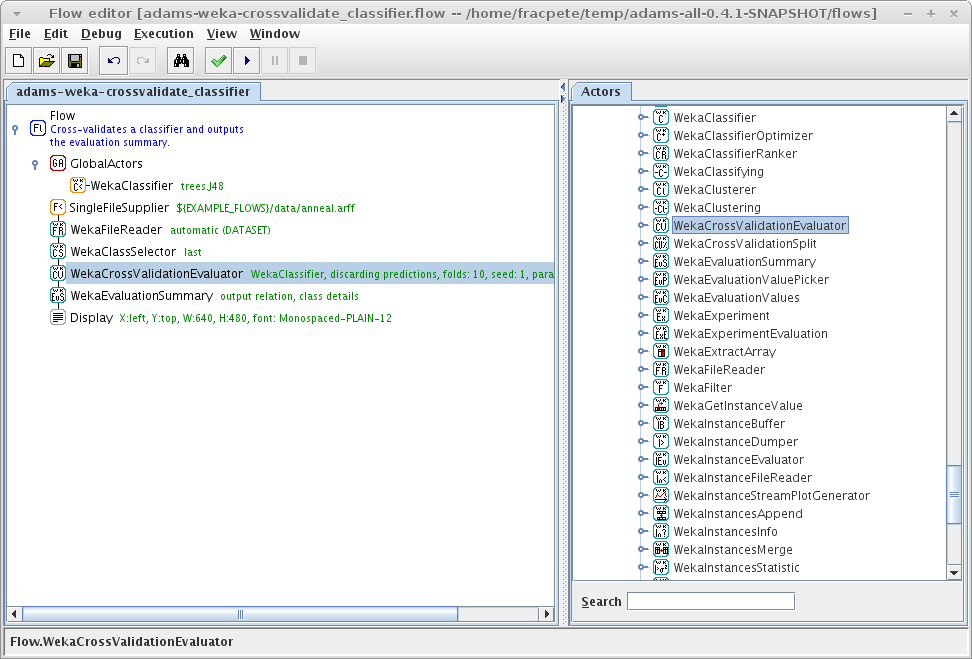
\includegraphics[width=6.0cm]{images/basic-crossvalidate1-flow.png}
    \caption{Cross-validating a classifier and outputting the summary.}
    \label{basic-crossvalidate1-flow}
  \end{minipage}
  \hspace{0.5cm}
  \begin{minipage}[t]{0.5\linewidth}
    \centering
    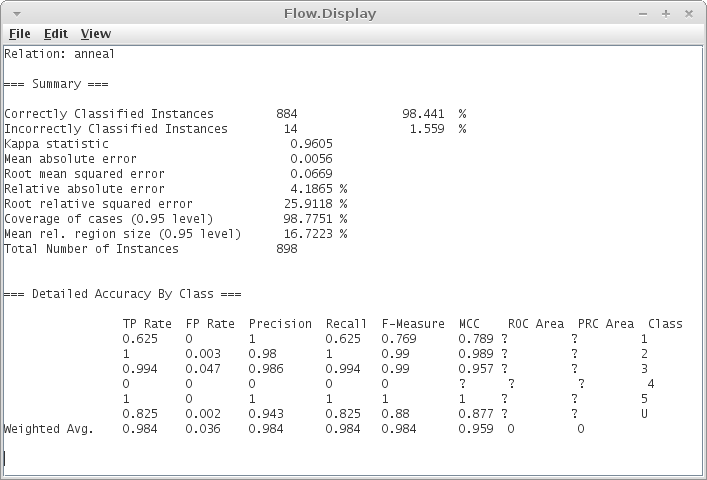
\includegraphics[width=5.5cm]{images/basic-crossvalidate1-output.png}
    \caption{Summary output of a cross-validated classifier.}
    \label{basic-crossvalidate1-output}
  \end{minipage}
\end{figure}

Most of the time, you don't just want to test a single classifier, but several
ones. With ADAMS you can, for instance, load classifier command-lines from a
text file and then evaluate them one after the
after\footnote{adams-weka-crossvalidate\_classifier\_setups\_from\_text\_file.flow}.
Reading the text file (see Figure
\ref{basic-crossvalidate_multiple_files-setups}) is fairly straight-forward,
using the \textit{TextFileReader} transformer.

\begin{figure}[htb]
  \centering
  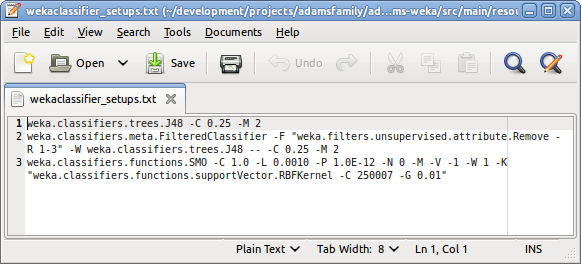
\includegraphics[width=6.0cm]{images/basic-crossvalidate_multiple_files-setups.png}
  \caption{Text file with command-lines of various classifiers.}
  \label{basic-crossvalidate_multiple_files-setups}
\end{figure}

For updating the callable classifier's set up, we need to attach a variable to the
callable \textit{WekaClassifierSetup} actor's ``classifier'' option and update this
variable with each set up that we are reading from the text file using the
\textit{SetVariable} transformer. This update of the classifier set up has to
happen before we are triggering the cross-validation. Figures
\ref{basic-crossvalidate_multiple_files-flow} and
\ref{basic-crossvalidate_multiple_files-output} show the full flow and the
generated output, when reading in three set ups from a text file (J48,
filtered J48, SMO).

\begin{figure}[ht]
  \begin{minipage}[t]{0.5\linewidth}
    \centering
    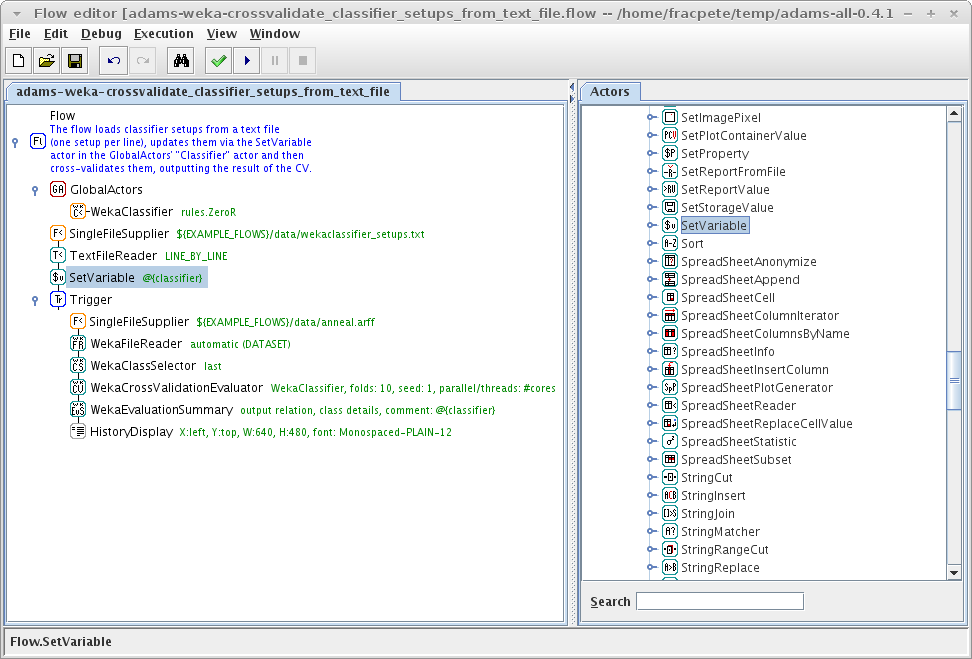
\includegraphics[width=6.0cm]{images/basic-crossvalidate_multiple_files-flow.png}
    \caption{Cross-validating classifier set ups read from a text file and
    displaying the evaluation summaries.}
    \label{basic-crossvalidate_multiple_files-flow}
  \end{minipage}
  \hspace{0.5cm}
  \begin{minipage}[t]{0.5\linewidth}
    \centering
    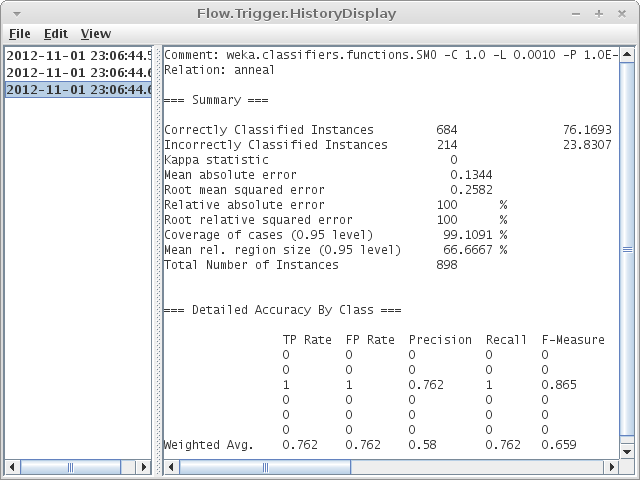
\includegraphics[width=5.5cm]{images/basic-crossvalidate_multiple_files-output.png}
    \caption{Summary outputs of cross-validated classifiers.}
    \label{basic-crossvalidate_multiple_files-output}
  \end{minipage}
\end{figure}

\heading{Test set evaluation}
Simply testing a built classifier on a test set is useful when you are always
intending to save the generated model to a file, but also want to keep an eye on
the performance. In this case, you can very easily extend your current flow for
building and saving the model. First, add a callable actor that loads the separate
training set from disk. Second, add a \textit{Tee} control actor that performs
the evaluation using the \textit{WekaTestSetEvaluator} and
\textit{WekaEvaluationSummary} transformers and a \textit{Display} sink for
showing the
results\footnote{adams-weka-build\_classifier\_evaluate\_on\_testset.flow}. The
full flow and the generated output are shown in Figures
\ref{basic-testseteval-flow} and \ref{basic-testseteval-output}.

\begin{figure}[ht]
  \begin{minipage}[t]{0.5\linewidth}
    \centering
    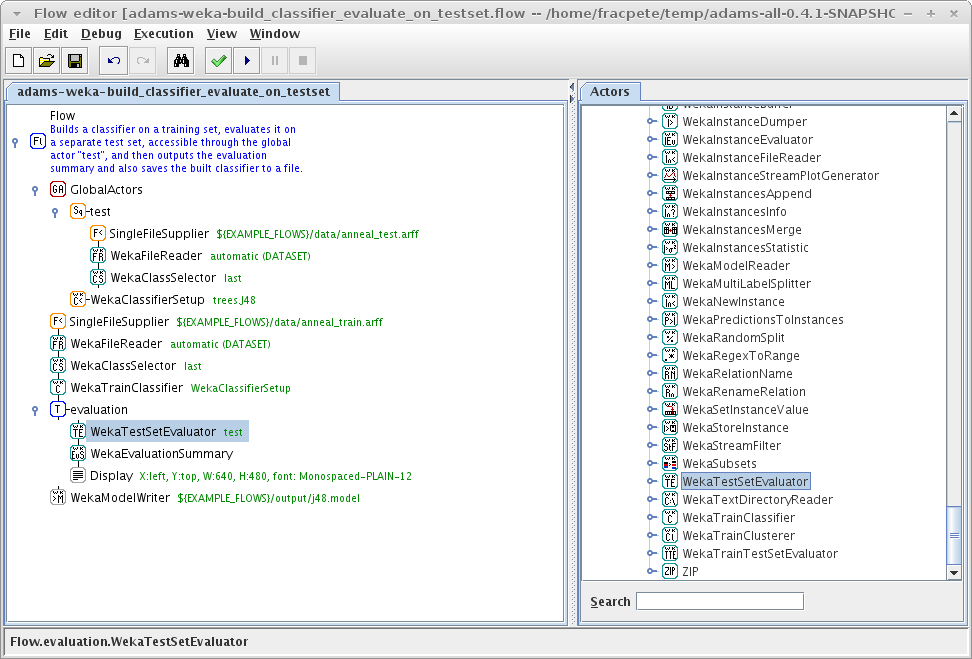
\includegraphics[width=6.0cm]{images/basic-testseteval-flow.png}
    \caption{Flow for evaluating built classifier on a separate test set.}
    \label{basic-testseteval-flow}
  \end{minipage}
  \hspace{0.5cm}
  \begin{minipage}[t]{0.5\linewidth}
    \centering
    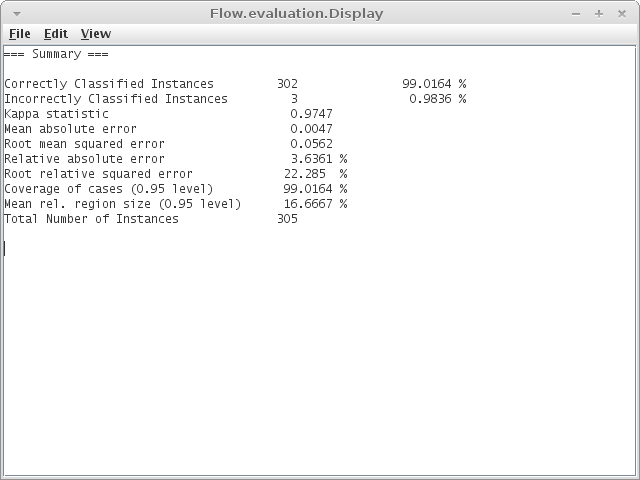
\includegraphics[width=5.5cm]{images/basic-testseteval-output.png}
    \caption{Summary output of classifier evaluated on separate test set.}
    \label{basic-testseteval-output}
  \end{minipage}
\end{figure}

\heading{Train/test set evaluation}
An evaluation using separate train and test set can be used, if you don't want
to keep the evaluated model, but you are only interested in the evaluation
output. The evaluation actor in this case is the
\textit{WekaTrainTestSetEvaluator} transformer. This actor accepts
\textit{WekaTrainTestSetContainer} data tokens. To generate this container you
have several options:
\begin{tight_itemize}
	\item \textit{WekaRandomSplit} -- splits a single dataset into a train and test
	set, based on the percentage supplied by the user.
	\item \textit{WekaCrossValidationSplit} -- Generates train/test splits like
	they occur in cross-validation. Useful, if you want to inspect the various models
	built during cross-validation, not just the summary.
	\item \textit{MakeContainer} -- manually generating a container from two
	individually loaded datasets.
\end{tight_itemize}

Figures \ref{basic-randomspliteval-flow} and \ref{basic-randomspliteval-output}
show how to use the \textit{RandomSplit} actor in the evaluation
process\footnote{adams-weka-evaluate\_classifier\_randomsplit.flow}. For
simulating cross-validation, simply exchange the \textit{WekaRandomSplit} actor
with a \textit{WekaCrossValidationSplit} one (you might also want to change from
\textit{Display} to \textit{HistoryDisplay}, to keep better track of the various
evaluations).

\begin{figure}[ht]
  \begin{minipage}[t]{0.5\linewidth}
    \centering
    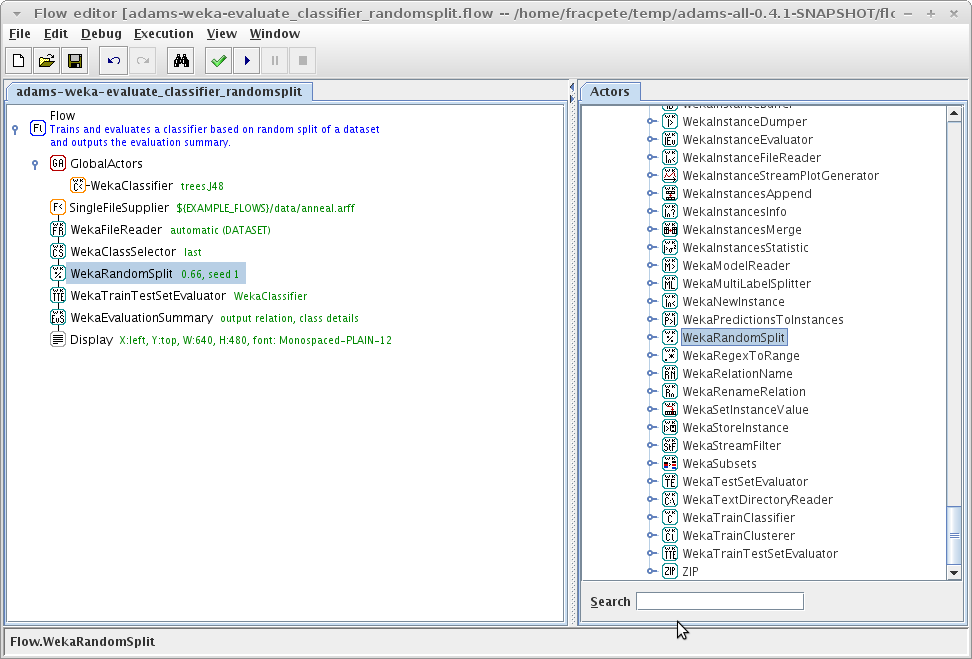
\includegraphics[width=6.0cm]{images/basic-randomspliteval-flow.png}
    \caption{Flow for building/evaluating classifier on a random split.}
    \label{basic-randomspliteval-flow}
  \end{minipage}
  \hspace{0.5cm}
  \begin{minipage}[t]{0.5\linewidth}
    \centering
    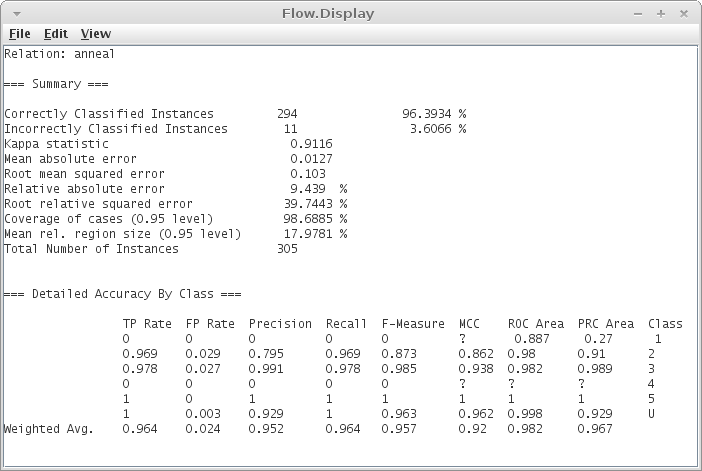
\includegraphics[width=5.5cm]{images/basic-randomspliteval-output.png}
    \caption{Summary output of classifier built/evaluated on random split.}
    \label{basic-randomspliteval-output}
  \end{minipage}
\end{figure}

Figures \ref{basic-traintestseteval-flow} and
\ref{basic-traintestseteval-output} display the flow\footnote{adams-weka-assemble\_traintestset\_container\_and\_evaluate\_classifier.flow}
for manually creating a container using the general purpose
\textit{MakeContainer} source actor. In order to assemble a container, you need
to know \textbf{what} type of container you want to create (the type is normally
listed in the ``Help'' of an actor), \textbf{where} to obtain the data from
(i.e., the callable actors) and \textbf{how} to store the data (i.e., under which
name in the container).

\begin{figure}[ht]
  \begin{minipage}[t]{0.5\linewidth}
    \centering
    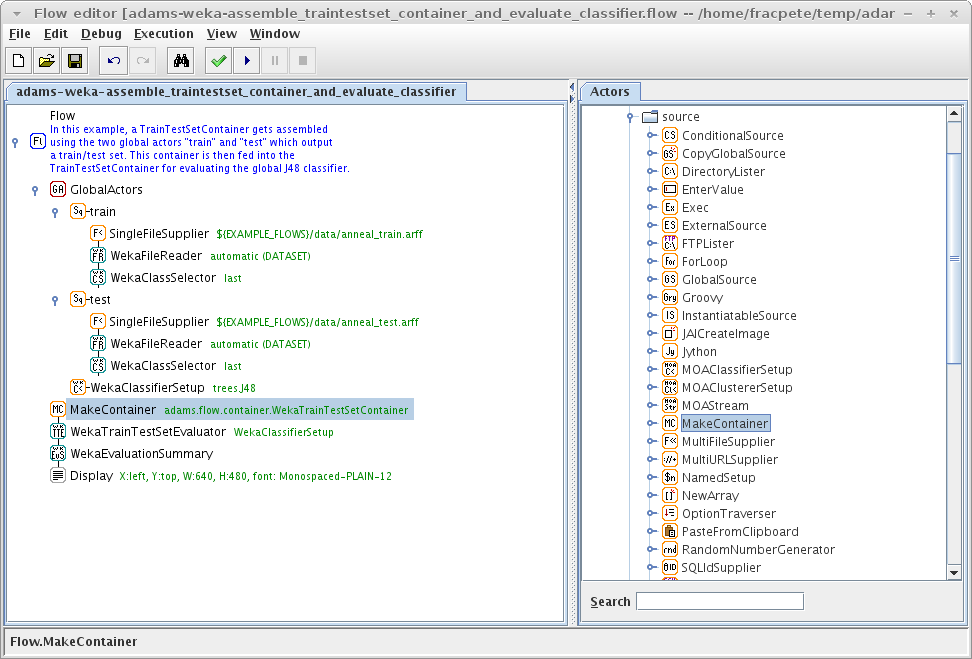
\includegraphics[width=6.0cm]{images/basic-traintestseteval-flow.png}
    \caption{Flow for evaluating classifier on separate train/test set.}
    \label{basic-traintestseteval-flow}
  \end{minipage}
  \hspace{0.5cm}
  \begin{minipage}[t]{0.5\linewidth}
    \centering
    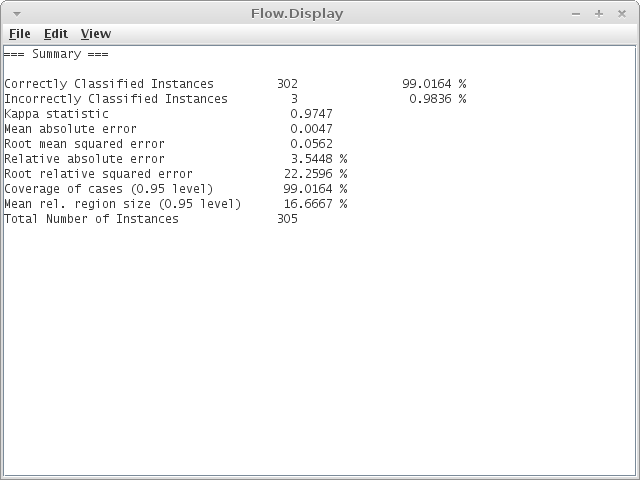
\includegraphics[width=5.5cm]{images/basic-traintestseteval-output.png}
    \caption{Summary output of classifier evaluated on separate train/test set.}
    \label{basic-traintestseteval-output}
  \end{minipage}
\end{figure}

\heading{Stream evaluation}
Though WEKA is usually used for batch-training, it is also possible to perform
incremental training and evaluation, as long as the classifier in use is an
\textit{updateable} one (i.e., it implements the \textit{weka.classifiers.Updateable}
interface). In such a scenario, you only have to read in the data incrementally
(changing the set up in the \textit{WekaFileReader} to \textit{INCREMENTAL})
and use the \textit{WekaStreamEvaluator} transformer for performing the
evaluation. The \textit{WekaStreamEvaluator} actor use prequential evaluation,
i.e., first evaluate, then train. Figure \ref{basic-streameval-flow} shows a 
flow that evaluates a \textit{NaiveBayesUpdateable} on a stream of data, 
displaying the textual evaluation summary and ROC (receiver operator curve) 
every 100 instances that come through.

\begin{figure}[ht]
  \begin{minipage}[t]{0.5\linewidth}
    \centering
    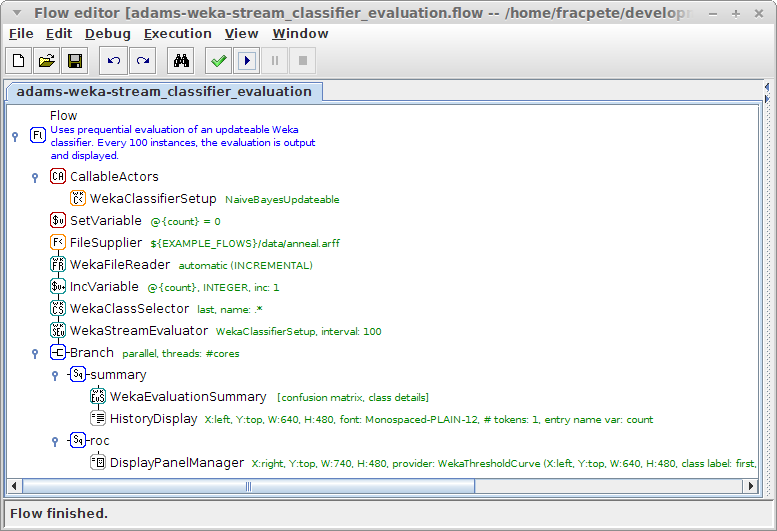
\includegraphics[width=10.0cm]{images/basic-streameval-flow.png}
    \caption{Flow for evaluating updateable classifier on data stream.}
    \label{basic-streameval-flow}
  \end{minipage}
\end{figure}

\begin{figure}[ht]
  \begin{minipage}[t]{0.5\linewidth}
    \centering
    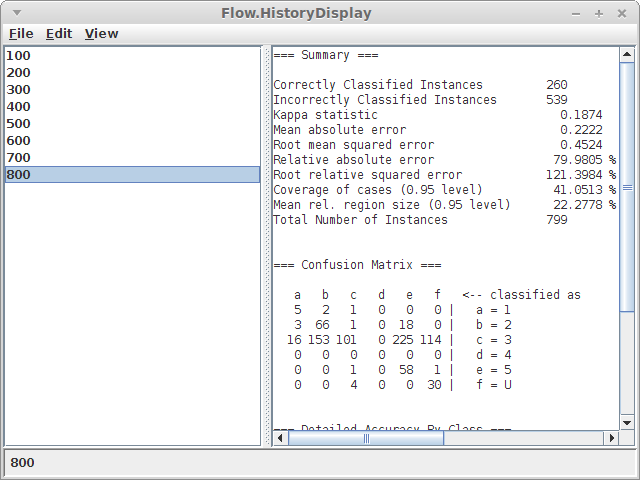
\includegraphics[width=5.5cm]{images/basic-streameval-output.png}
    \caption{Summary output of classifier evaluated on data stream.}
    \label{basic-streameval-output}
  \end{minipage}
  \hspace{0.5cm}
  \begin{minipage}[t]{0.5\linewidth}
    \centering
    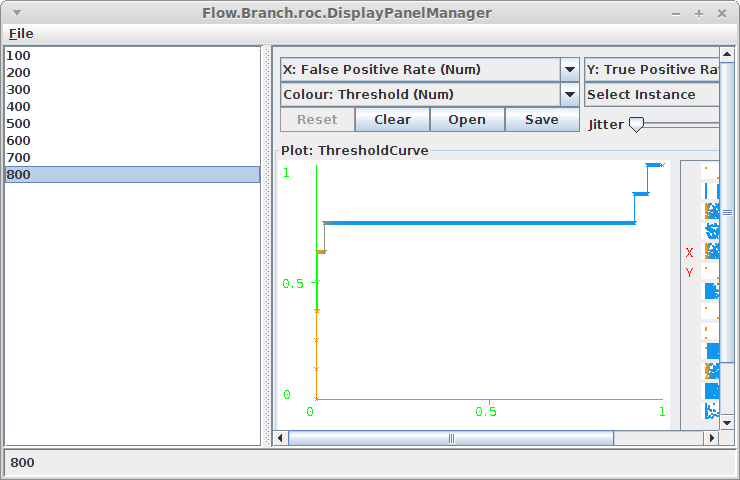
\includegraphics[width=5.5cm]{images/basic-streameval-output2.png}
    \caption{ROC curves of classifier evaluated on data stream.}
    \label{basic-streameval-output2}
  \end{minipage}
\end{figure}


\heading{Visualization}
You have already encountered the display of the classifier errors (in Figure
\ref{basic-preprocessing_errors-original}). The sink for displaying these errors
is \textit{WekaClassifierErrors}, which takes an \textit{Evaluation} object as
input. If you want to evaluate and display multiple classifiers then you have to
use the \textit{DisplayPanelManager} with the \textit{WekaClassifierErrors}
actor as ``panelProvider''. The \textit{DisplayPanelManager} actor offers a
history of generated panels, like the \textit{HistoryDisplay} does for plain
text.

Another interesting visualization is the \textit{WekaAccumulatedError}
transformer. This transformer takes also an \textit{Evaluation} object and then
turns it into a special sequence of plot containers: it creates a sequence of
the prediction errors that were obtained during an evaluation and outputs them
sorted, from smallest to
largest\footnote{adams-weka-accumulated\_error\_display.flow}. The Figures
\ref{basic-accumulatederror-flow} and \ref{basic-accumulatederror-output} show
the flow and the generated output respectively. As you can see from the graph,
GaussianProcesses generates consistently larger errors than LinearRegression,
which only seems to have a few big outliers (steep increase at the end).

\begin{figure}[ht]
  \begin{minipage}[t]{0.5\linewidth}
    \centering
    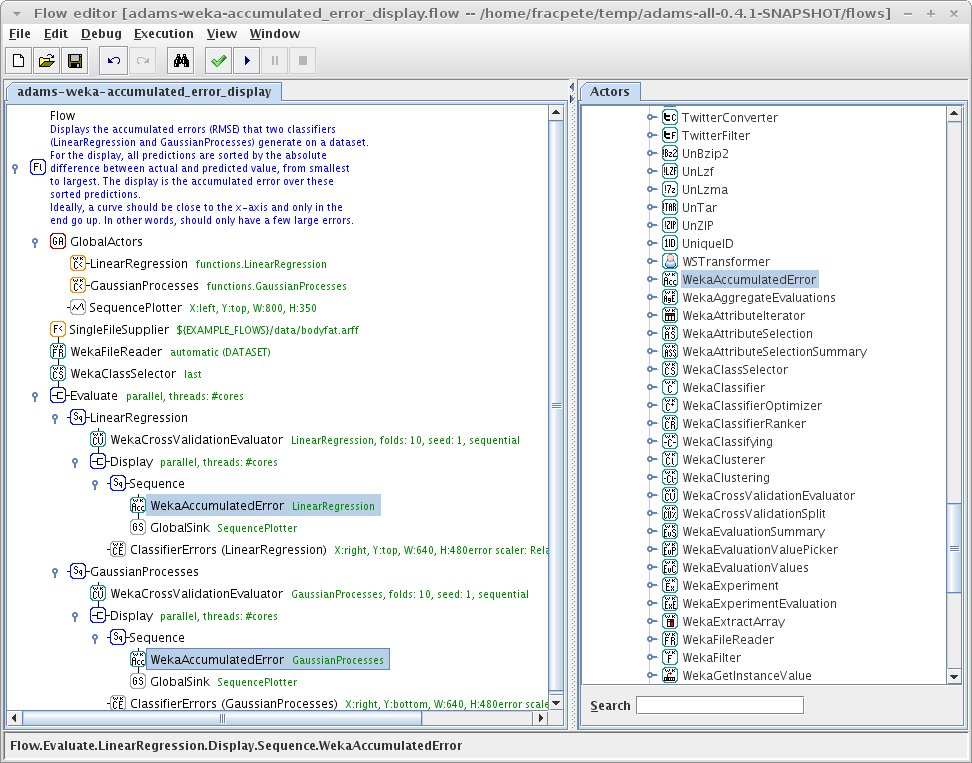
\includegraphics[width=6.0cm]{images/basic-accumulatederror-flow.png}
    \caption{Flow for displaying the ``accumulated error'' of a two
    classifiers.}
    \label{basic-accumulatederror-flow}
  \end{minipage}
  \hspace{0.5cm}
  \begin{minipage}[t]{0.5\linewidth}
    \centering
    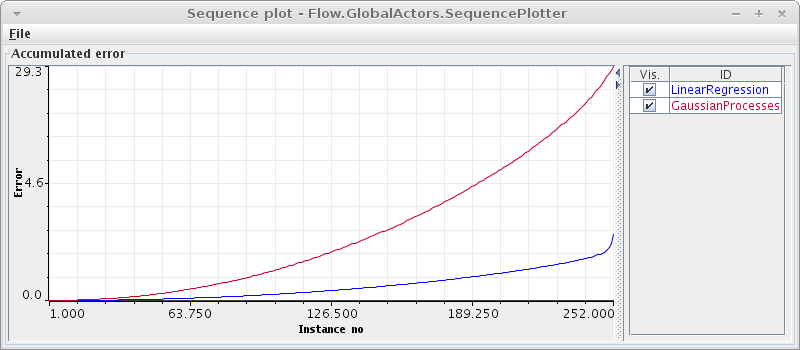
\includegraphics[width=5.5cm]{images/basic-accumulatederror-output.png}
    \caption{The ``accumulated error'' of LinearRegression and
    GaussianProcesses.}
    \label{basic-accumulatederror-output}
  \end{minipage}
\end{figure}

\clearpage
\subsection{Making predictions}
Of course, building models is only part of the picture. You will want to use
this model as well and make predictions with it. The actor for making
predictions on incoming data (i.e., single instance objects) is the
\textit{WekaClassifying} actor. This actor can either use a serialized model or
a callable actor that generates a trained classifier. The
flow\footnote{adams-weka-classifying\_data.flow} in Figure
\ref{basic-classifying-flow} uses the callable actor approach, training a
classifier on a training set and then performing classifications on a test set,
with the class distributions shown on screen (see Figure
\ref{basic-classifying-output}).

\begin{figure}[ht]
  \begin{minipage}[t]{0.5\linewidth}
    \centering
    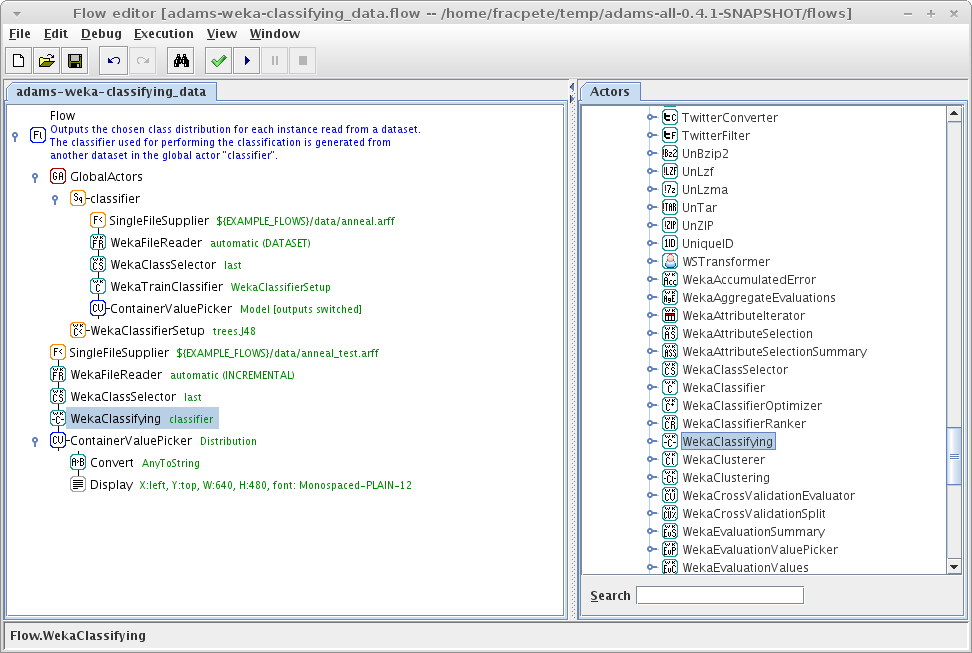
\includegraphics[width=6.0cm]{images/basic-classifying-flow.png}
    \caption{Flow for classifying new data and outputting the class
    distributions.}
    \label{basic-classifying-flow}
  \end{minipage}
  \hspace{0.5cm}
  \begin{minipage}[t]{0.5\linewidth}
    \centering
    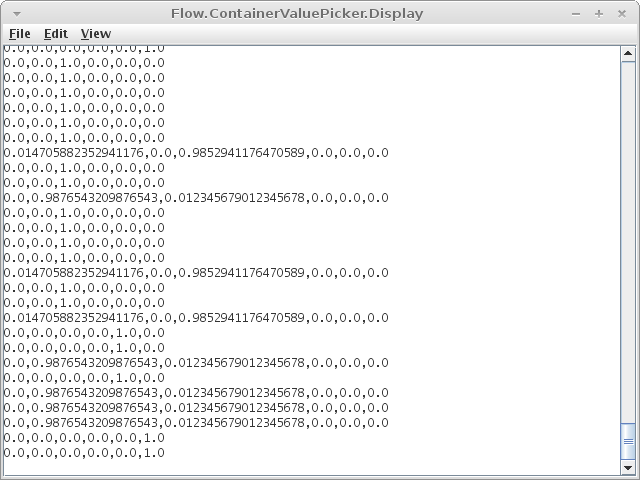
\includegraphics[width=5.5cm]{images/basic-classifying-output.png}
    \caption{The generated class distributions for the new data.}
    \label{basic-classifying-output}
  \end{minipage}
\end{figure}

\newpage
\section{Advanced}

\subsection{Learning curves}
Classifiers are susceptible to the order and amount of data that they are
trained with. Using learning curves, one can investigate how the data
influences the classifier performance.

Figures \ref{advanced-learning_curve-incremental-flow} and \ref{advanced-learning_curve-incremental-output}
show a flow and the generated output of an incremental NaiveBayes classifier, 
with the classifier being evaluated against a test set every 10 training 
instances (\textit{ConditionalTee} in conjunction with the \textit{Counting}
condition).\footnote{adams-weka-build\_classifier\_incrementally.flow}

\begin{figure}[ht]
  \begin{minipage}[t]{0.55\linewidth}
    \centering
    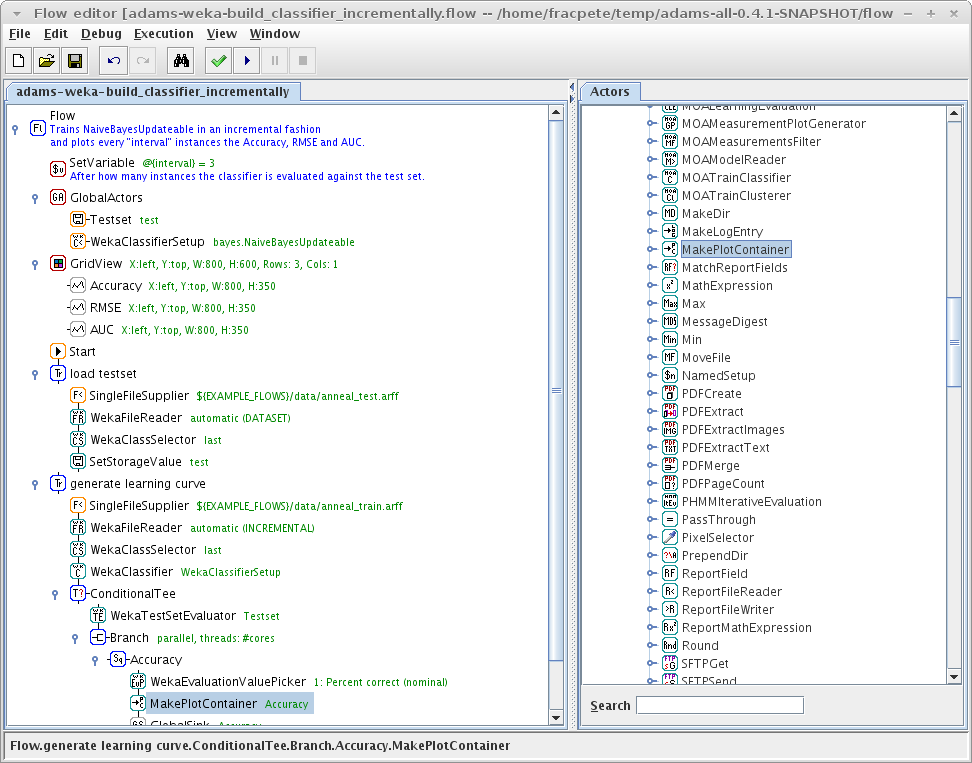
\includegraphics[width=7.0cm]{images/advanced-learning_curve-incremental-flow.png}
    \caption{Flow for generating learning curve for incremental classifier.}
    \label{advanced-learning_curve-incremental-flow}
  \end{minipage}
  \hspace{0.5cm}
  \begin{minipage}[t]{0.45\linewidth}
    \centering
    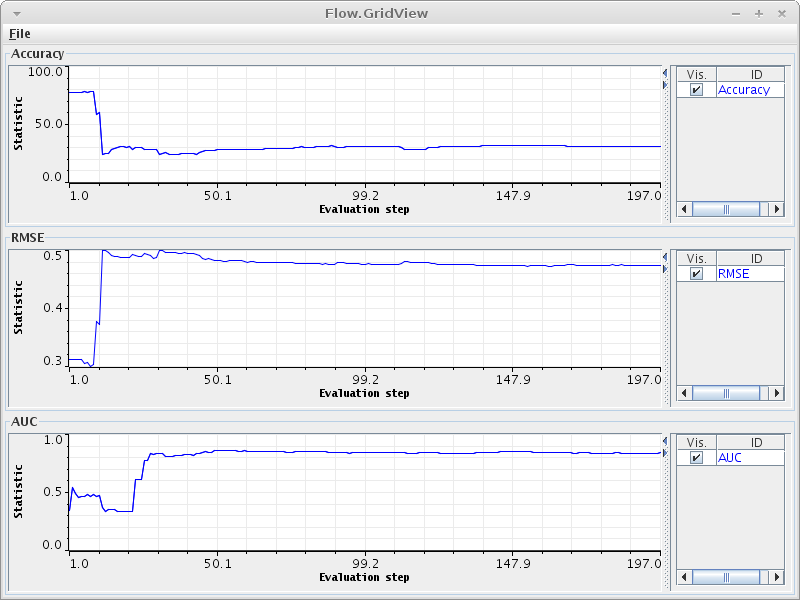
\includegraphics[width=4.5cm]{images/advanced-learning_curve-incremental-output.png}
    \caption{Generated learning curve (incremental).}
    \label{advanced-learning_curve-incremental-output}
  \end{minipage}
\end{figure}

Incremental classifiers are great for generating these kind of graphs. But
even for batch classifiers you can generate learning curves. Using the 
\textit{WekaInstanceBuffer} transformer, it is possible to buffer instances as
they come through and output datasets with which the batch classifer can get
trained (and evaluated). Figures \ref{advanced-learning_curve-batch-flow} and
\ref{advanced-learning_curve-incremental-output} show how to generate a 
learning curve for the decision tree classifier J48, being evaluated every
10 instances.\footnote{adams-weka-classifier\_learning\_curve.flow}

\begin{figure}[ht]
  \begin{minipage}[t]{0.55\linewidth}
    \centering
    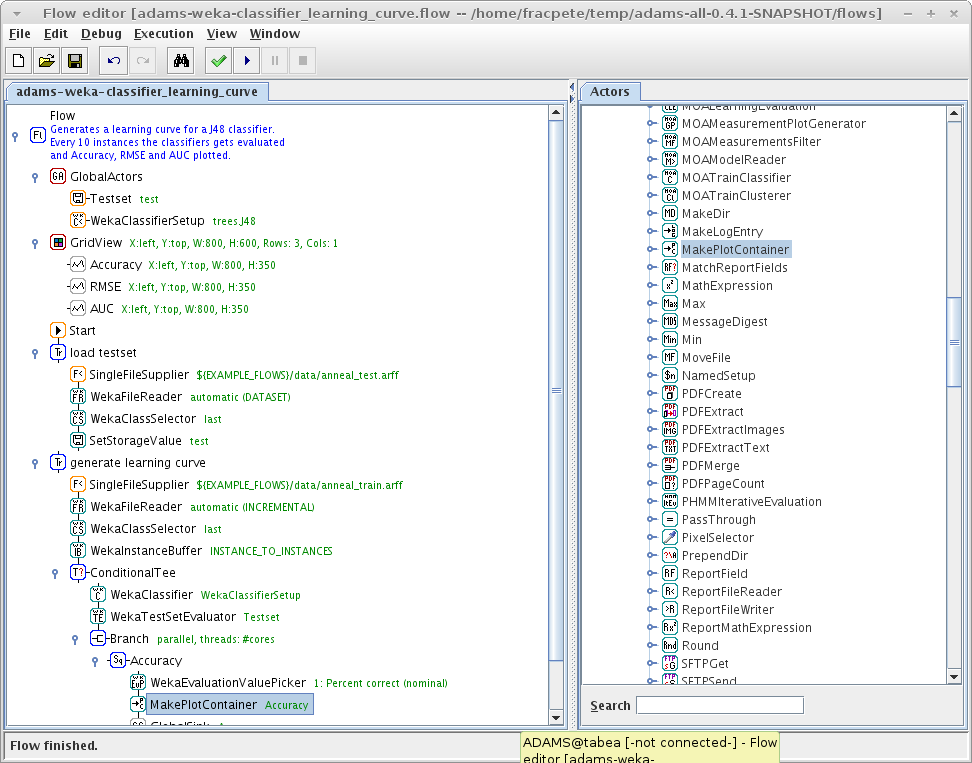
\includegraphics[width=7.0cm]{images/advanced-learning_curve-batch-flow.png}
    \caption{Flow for generating learning curve for batch classifier.}
    \label{advanced-learning_curve-batch-flow}
  \end{minipage}
  \hspace{0.5cm}
  \begin{minipage}[t]{0.45\linewidth}
    \centering
    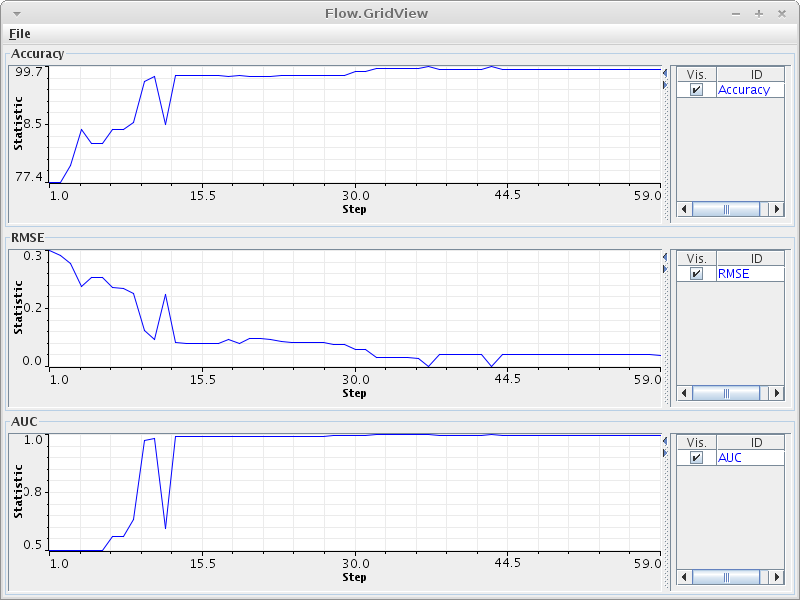
\includegraphics[width=4.5cm]{images/advanced-learning_curve-batch-output.png}
    \caption{Generated learning curve (batch).}
    \label{advanced-learning_curve-batch-output}
  \end{minipage}
\end{figure}

\subsection{Experiments}
experiment generation\footnote{adams-weka-experiment\_generation.flow},
execution and evaluation\footnote{adams-weka-experiment.flow}

\subsection{Optimization}
setup generators\footnote{adams-weka-classifier\_setup\_generation.flow},
ranker\footnote{adams-weka-classifier\_setup\_ranking.flow},
optimizer\footnote{adams-weka-classifier\_optimizer.flow}

\subsection{Provenance}
Machine learning related actors can keep track of what operations happened
along the way, or in other words, provenance.

Due to the additional load, provenance is turned off by default. You can turn
it on by placing a properties file called \texttt{Provenance.props}
home directory with the following content:
\begin{verbatim}
Enabled=true
\end{verbatim}

Figure \ref{advanced-provenance-flow} shows the flow that cross-validates a
classifier on a pre-processed dataset. The provenance trace of loading
the data, pre-processing and evaluating it, can be seen in Figure 
\ref{advanced-provenance-output}.

\begin{figure}[ht]
  \begin{minipage}[t]{0.55\linewidth}
    \centering
    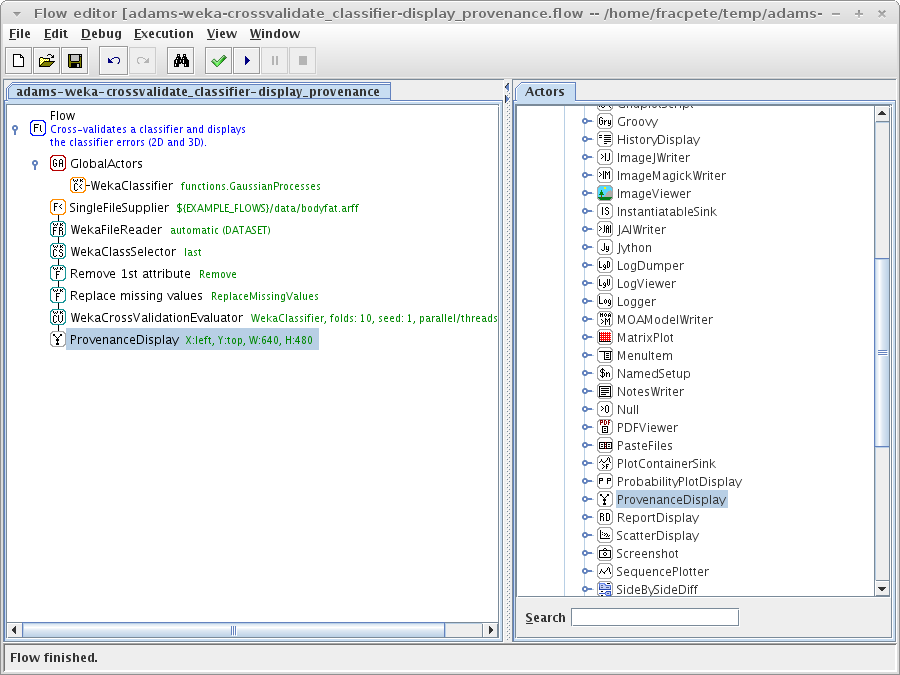
\includegraphics[width=7.0cm]{images/advanced-provenance-flow.png}
    \caption{Flow for cross-validating a classifier on a pre-processed dataset.}
    \label{advanced-provenance-flow}
  \end{minipage}
  \hspace{0.5cm}
  \begin{minipage}[t]{0.45\linewidth}
    \centering
    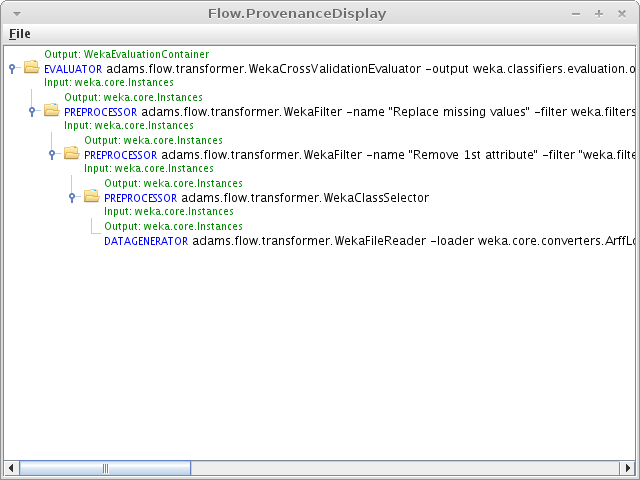
\includegraphics[width=4.5cm]{images/advanced-provenance-output.png}
    \caption{Provenance display.}
    \label{advanced-provenance-output}
  \end{minipage}
\end{figure}

provenance
display\footnote{adams-weka-crossvalidate\_classifier-display\_provenance.flow}

\subsection{Partial Least Squares}
Using the \textit{WekaExtractPLSMatrix} transformer, you can extract various
PLS matrices from a \textit{PLSFilterWithLoadings} filter or a 
\textit{PLSClassifierWeightedWithLoadings} classifier (or a \textit{WekaModelContainer},
if this container should have a \textit{PLSClassifierWeightedWithLoadings} classifier 
stored).\footnote{adams-weka-extract\_pls\_matrix.flow}
